\newpage
\begin{appendices}

\section{Q2}\label{app:Q2}

\subsection{2C}

\begin{figure}[!h]
  \centering
  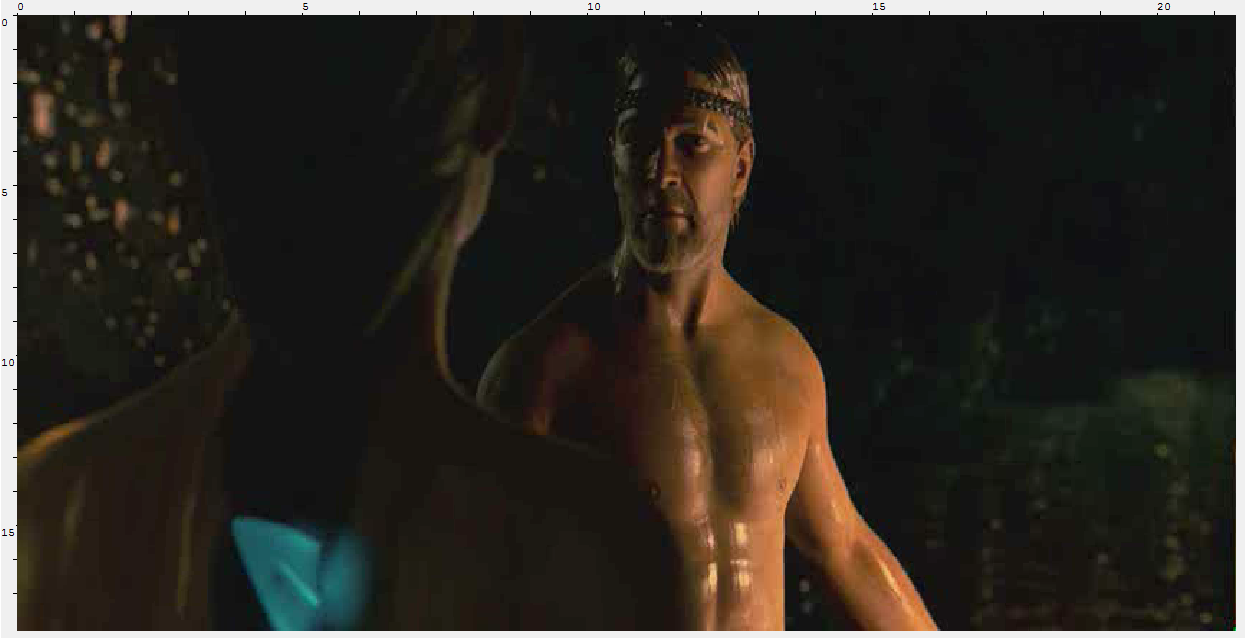
\includegraphics[width=\textwidth]{2C_mistakes_prior}
  \caption{Frame prior to concealed frame taken from the solution to exercice 2C (edge detection).} 
  \label{fig:2C_prior}
\end{figure}

\begin{figure}[!h]
  \centering
  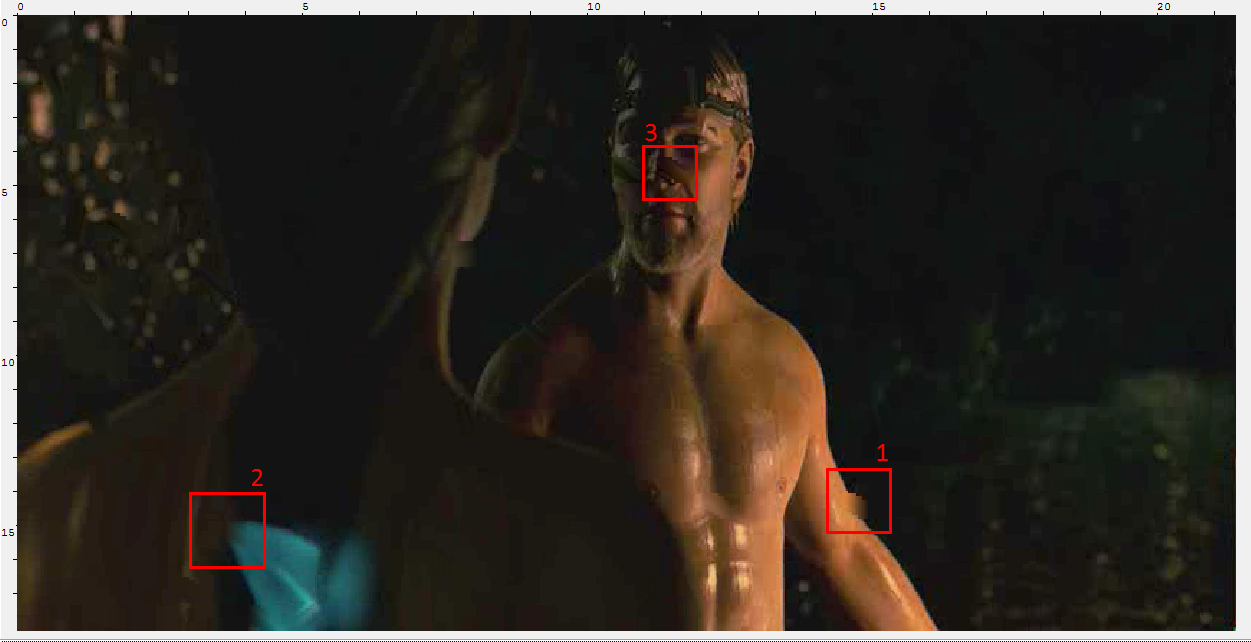
\includegraphics[width=\textwidth]{2C_mistakes}
  \caption{Concealed frame taken from the solution to exercice 2C (edge detection).} 
  \label{fig:2C}
\end{figure}

\newpage

\section{Q3: Timings}\label{Q3:timings}
\begin{table}[h]
\begin{tabular}{|l|l|l|l|l|l|}
\hline
\textbf{Frame}           & \textbf{AVG (s/frame)} & \textbf{total} & \textbf{PSNR} & \textbf{SSIM} & \textbf{AVG (fps)} \\ \hline
\textbf{2A simple}       & 0,000857               & 0,132          & 38,58747      & 0,937994      & 1166,667           \\ \hline
\textbf{2A complex}      & 0,002474               & 0,381          & 22,52592      & 0,520955      & 404,1995           \\ \hline
\textbf{2B simple}       & 0,001299               & 0,2            & 39,74085      & 0,940161      & 770                \\ \hline
\textbf{2B complex}      & 0,299948               & 46,192         & 32,66869      & 0,898557      & 3,333911           \\ \hline
\textbf{2C simple}       & 0,012948               & 1,994          & 39,4913       & 0,938137      & 77,2317            \\ \hline
\textbf{2C complex}      & 10,41379               & 1603,724       & 32,11392      & 0,893201      & 0,096026           \\ \hline
\textbf{3A simple}       & 0,000506               & 0,078          & 39,28378      & 0,927515      & 1974,359           \\ \hline
\textbf{3A complex}      & 0,000844               & 0,13           & 35,46008      & 0,879678      & 1184,615           \\ \hline
\textbf{3B (2) simple}   & 0,010292               & 1,585          & 39,82269      & 0,933798      & 97,16088           \\ \hline
\textbf{3B (2) complex}  & 0,081987               & 12,626         & 35,36771      & 0,896592      & 12,19705           \\ \hline
\textbf{3B (4) simple}   & 0,009351               & 1,44           & 39,82269      & 0,933798      & 106,9444           \\ \hline
\textbf{3B (4) complex}  & 0,073208               & 11,274         & 35,36771      & 0,869592      & 13,65975           \\ \hline
\textbf{3B (8) simple}   & 0,007273               & 1,12           & 39,82269      & 0,933798      & 137,5              \\ \hline
\textbf{3B (8) complex}  & 0,071643               & 11,033         & 35,36771      & 0,896592      & 13,95813           \\ \hline
\textbf{3B (16) simple}  & 0,007156               & 1,102          & 39,82269      & 0,933798      & 139,7459           \\ \hline
\textbf{3B (16) complex} & 0,064987               & 10,008         & 35,36771      & 0,896592      & 15,38769           \\ \hline
\textbf{3C simple}       & 0,031623               & 4,87           & 39,82269      & 0,933798      & 31,62218           \\ \hline
\textbf{3C complex}      & 0,157032               & 24,183         & 35,47011      & 0,892084      & 6,36811            \\ \hline
\textbf{3D simple}       & 0,045922               & 7,072          & 39,82269      & 0,933798      & 21,77602           \\ \hline
\textbf{3D complex}      & 0,240383               & 37,019         & 35,36771      & 0,896592      & 4,160026           \\ \hline
\end{tabular}
\end{table}

\newpage

\section{Q4}\label{app:Q4}

\begin{figure}[!h]\label{fig:time_simple_pattern}
  \centering
  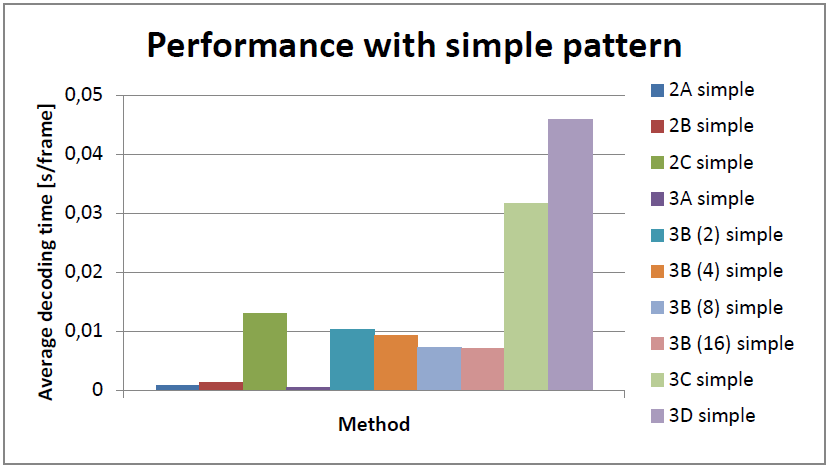
\includegraphics[width=.9\textwidth]{time_simple}
  \caption{Comparison of frame concealment time of all methods with the simple error pattern.} 
\end{figure}

\begin{figure}[!h]\label{fig:time_complex_pattern}
  \centering
  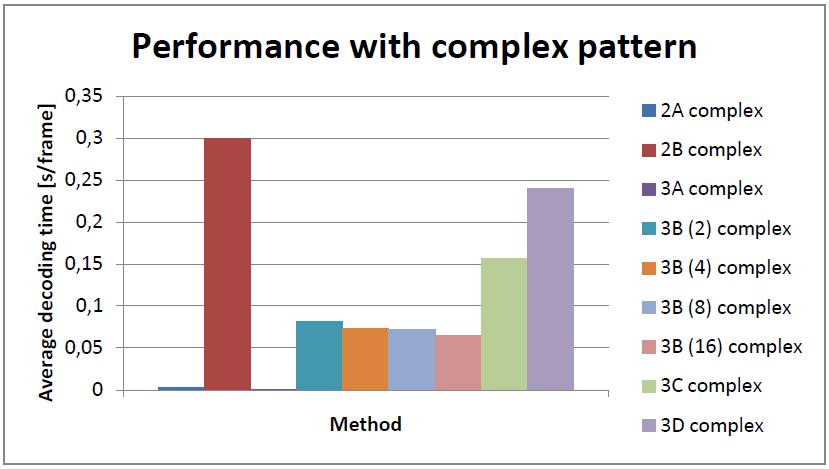
\includegraphics[width=.9\textwidth]{time_complex}
  \caption{Comparison of frame concealment time of all methods with the complex error pattern. The value of 2C has been left out, because it is too high (10,4138). This avoids that graph becomes unreadable.} 
\end{figure}

\newpage

\section{Q5}\label{Q5}
\subsection{Motion vectors}
\begin{figure}[!h]
  \centering
  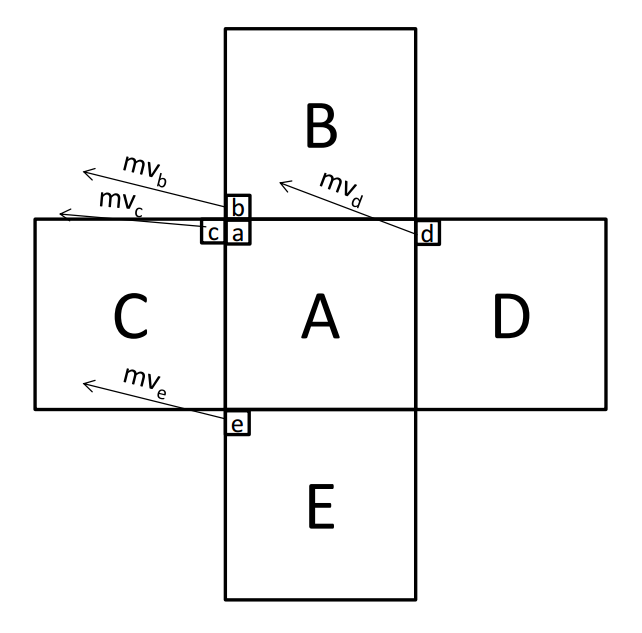
\includegraphics[width=.9\textwidth]{motions}
  \caption{The motions is consistent in the whole frame, therefore the calculated motion vector will be almost the same.} 
  \label{Q5:motions}
\end{figure}

\clearpage

\section{Q7}\label{Q7}
\subsection{Zero motion compared to motion estimation}
\begin{figure}[ht]
\centering
\begin{subfigure}{\textwidth}
  \centering
  
\includegraphics[width=.9\textwidth]{zero}
  \caption{zero motion}
\end{subfigure}\\
\begin{subfigure}{\textwidth}
  \centering
  
\includegraphics[width=.9\textwidth]{tweepertwee}
  \caption{Motion estimation with subblock of size 2}
\end{subfigure}
\caption{Zero motion (3A) compared with non-dynamic motion estimation (3B).}
\label{Q7:zerotwee}
\end{figure}

\clearpage

\subsection{Edges compated to motion estimation - simple pattern}
\begin{figure}[ht]
\centering
\begin{subfigure}{\textwidth}
  \centering
  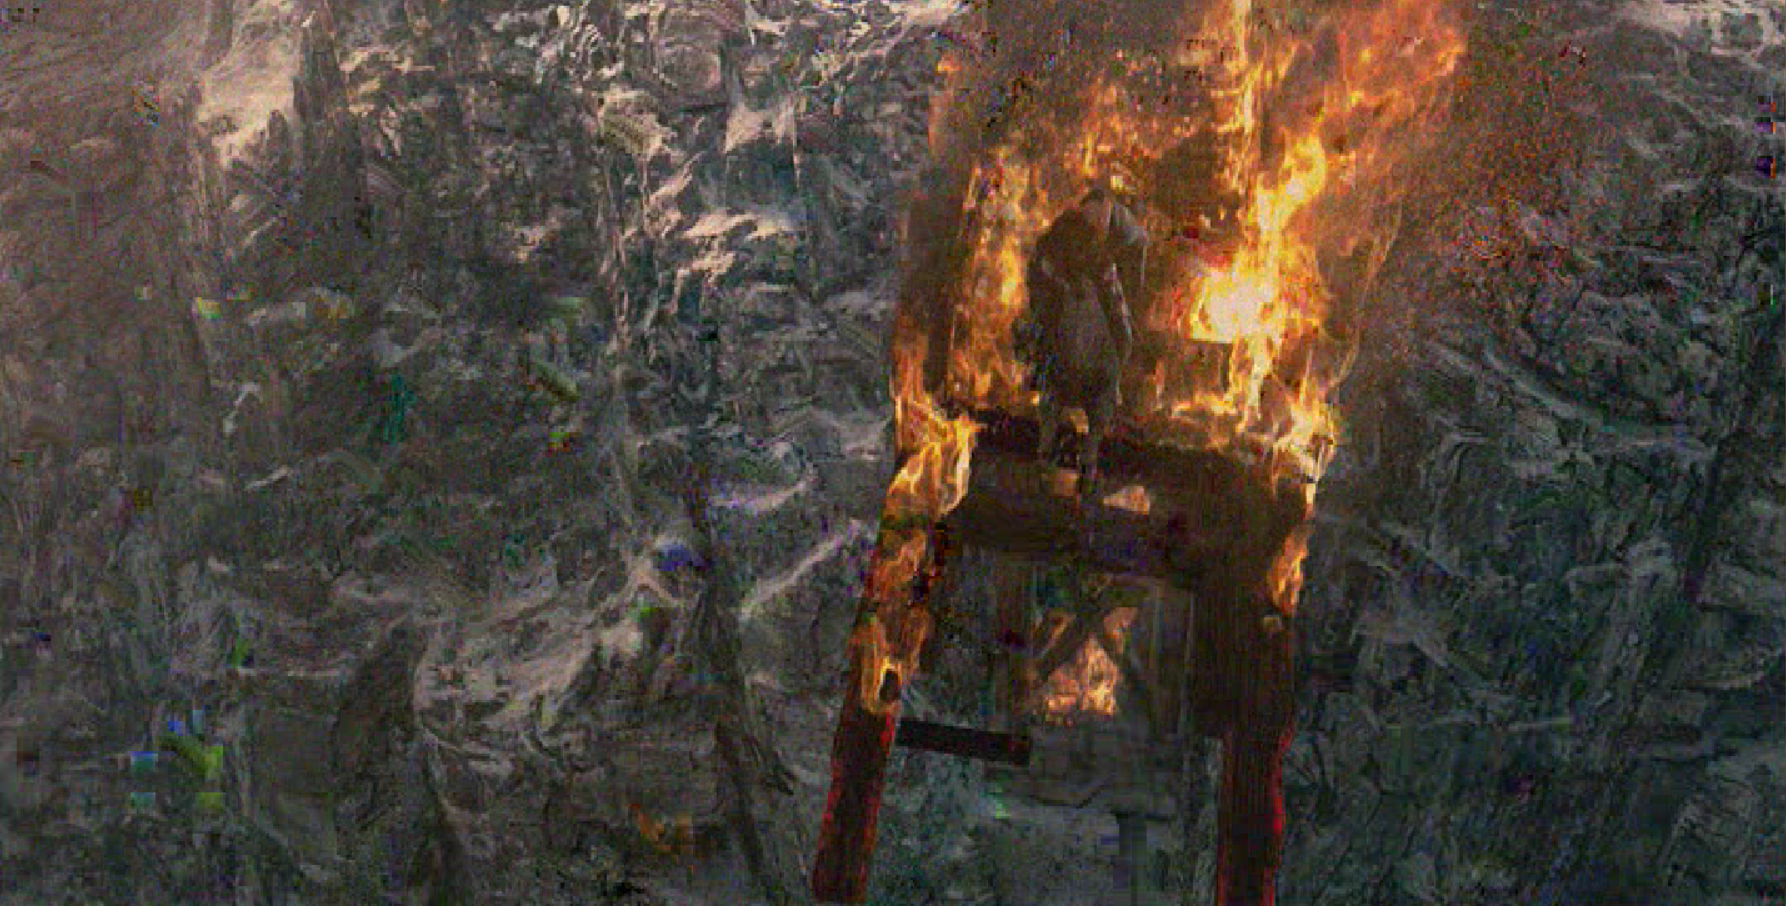
\includegraphics[width=.9\textwidth]{edges}
  \caption{Edge detection}
\end{subfigure}\\
\begin{subfigure}{\textwidth}
  \centering
  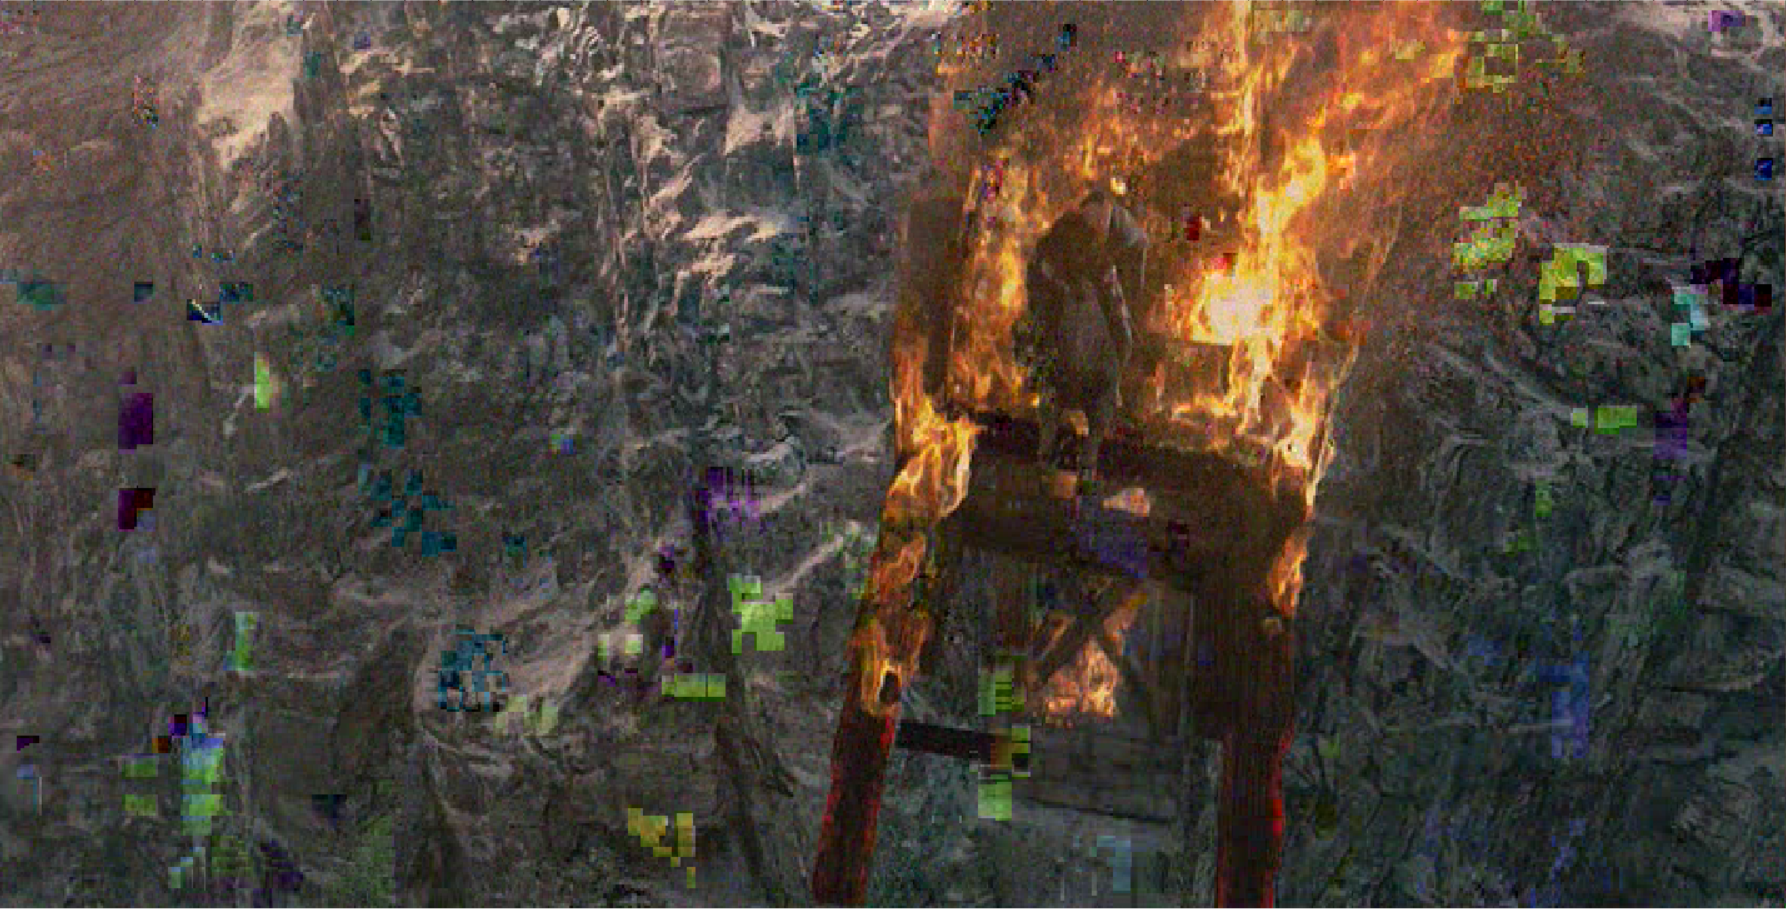
\includegraphics[width=.9\textwidth]{motion}
  \caption{Motion estimation with subblock of size 2}
\end{subfigure}
\caption{The simple pattern is better concealed with the spatial methods than the motion estimation.}
\label{Q7:edgemotion}
\end{figure}

\clearpage

\subsection{Edges compated to motion estimation - complex}
\begin{figure}[ht]
\centering
\begin{subfigure}{\textwidth}
  \centering
  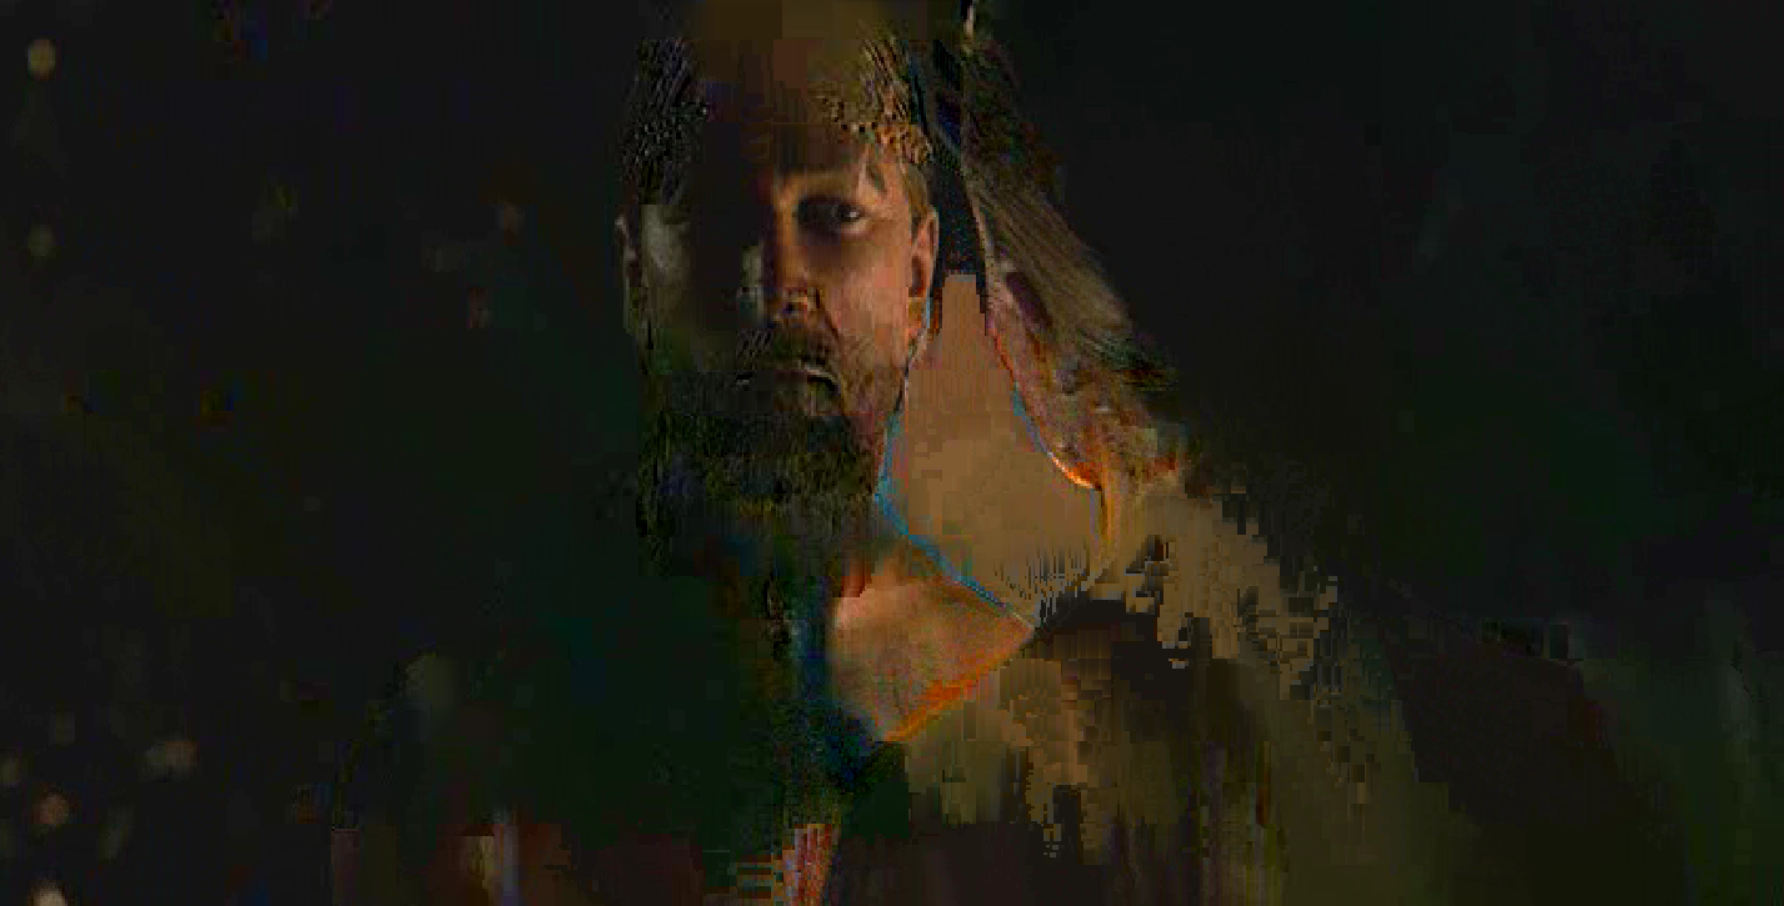
\includegraphics[width=.9\textwidth]{edgescomplex}
  \caption{Edge detection}
\end{subfigure}\\
\begin{subfigure}{\textwidth}
  \centering
  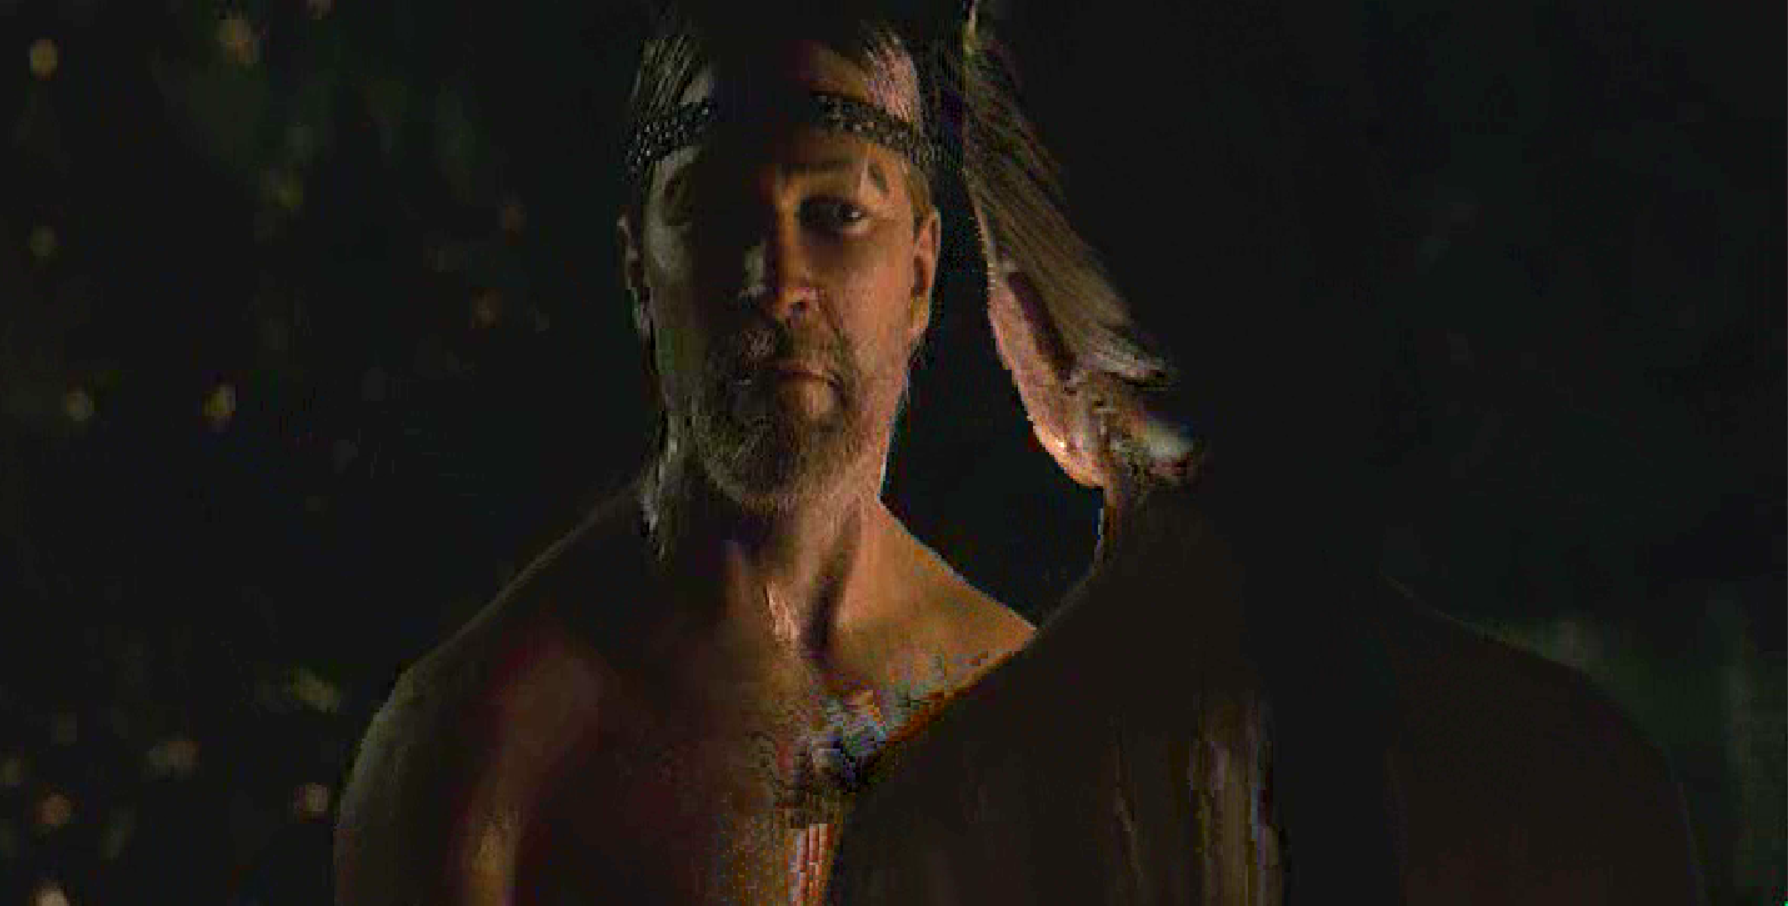
\includegraphics[width=.9\textwidth]{motioncomplex}
  \caption{Motion estimation with subblock of size 2}
\end{subfigure}
\caption{The complex pattern is better concealed with the motion estimation.}
\label{Q7:edgemotioncomplex}
\end{figure}

\newpage

\section{Q9}\label{app:Q9}
\begin{figure}[!h]\label{fig:PSNR_simple_pattern}
  \centering
  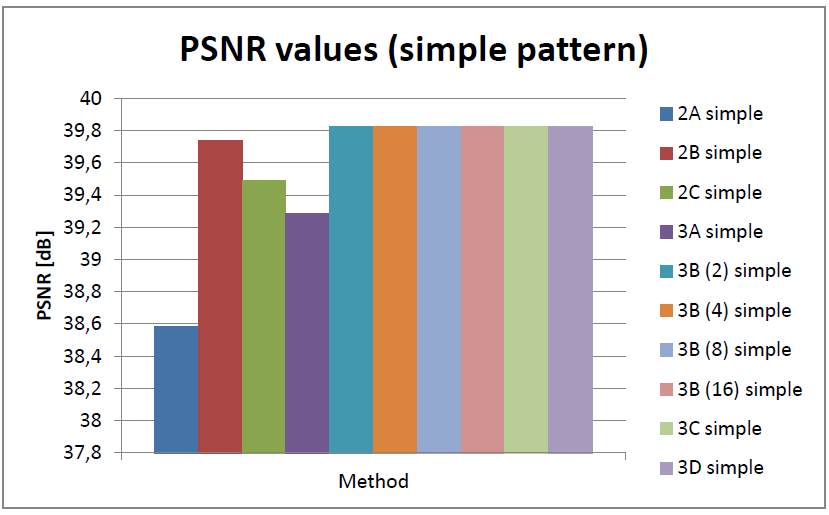
\includegraphics[width=.9\textwidth]{PSNR_simple}
  \caption{Comparison of PSNR values of all methods with the simple error pattern.} 
\end{figure}
\begin{figure}[!h]\label{fig:PSNR_complex_pattern}
  \centering
  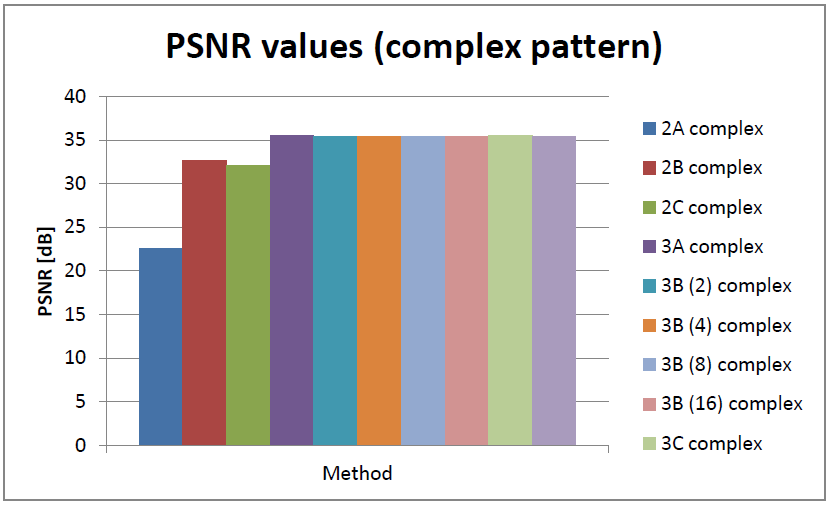
\includegraphics[width=.9\textwidth]{PSNR_complex}
  \caption{Comparison of PSNR values of all methods with the complex error pattern.} 
\end{figure}

\newpage

\section{Q10}\label{app:Q10}
\begin{figure}[!h]\label{fig:SSIM_simple_pattern}
  \centering
  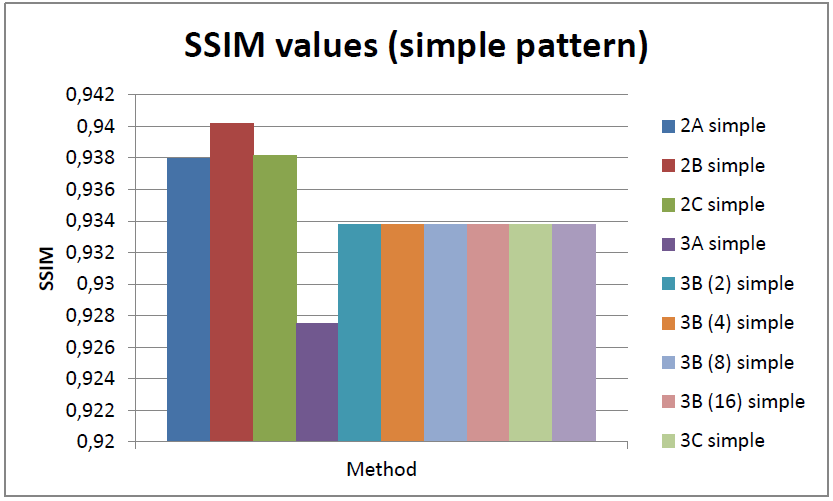
\includegraphics[width=.9\textwidth]{SSIM_simple}
  \caption{Comparison of SSIM values of all methods with the simple error pattern.} 
\end{figure}

\begin{figure}[!h]\label{fig:SSIM_complex_pattern}
  \centering
  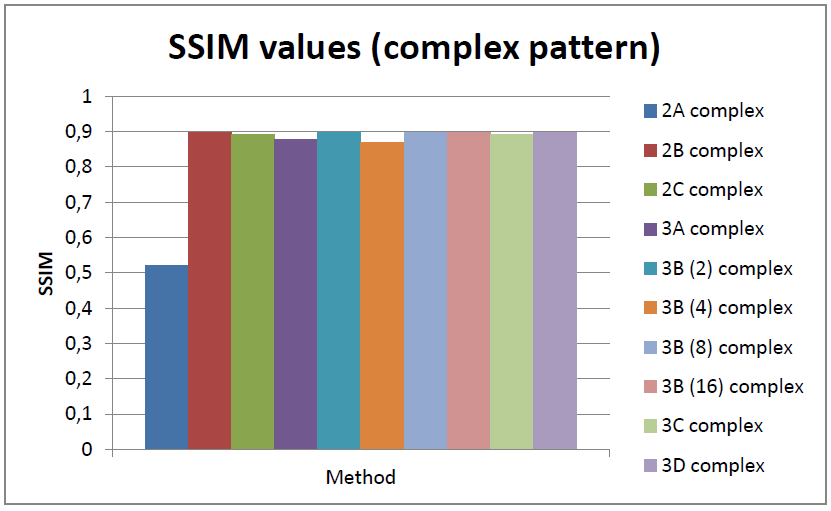
\includegraphics[width=.9\textwidth]{SSIM_complex}
  \caption{Comparison of SSIM values of all methods with the complex error pattern.} 
\end{figure}

\end{appendices}